Es gibt zwei unterschiedliche Arten von CAN-Telegrammen: die Standard-CAN-Frames (kurze Telegramme nach CAN-Spezifikation 2.0A) und die Extended-CAN-Frames (lange Telegramme nach CAN-Spezifikation 2.0B). Der wesentliche Unterschied zwischen diesen beiden Telegrammarten liegt in der Länge des CAN-Identifiers bzw. in der Anzahl der verfügbaren logischen Adressen. Beim Telegramm nach CAN-Spezifikation 2.0A ist der Identifier 11 Bits lang, sodass 2048 verschiedene logische Adressen möglich sind. Beim Telegramm nach CAN-Spezifikation 2.0B beträgt die Länge des Identifiers 29 Bits, was 536.870.912 logische Adressen ermöglicht. \cite{lawrenzCANControllerArea2016}

\subsection{Aufbau von kurzen CAN-Telegrammen}
Im folgenden Abschnitt wird zunächst der Aufbau eines kurzen Telegramms beschrieben, bevor im Anschluss auf die Besonderheiten des langen Telegramms eingegangen wird. Ein CAN-Telegramm lässt sich in unterschiedliche Abschnitte bzw. Felder unterteilen. 

    \begin{figure}[htbp]
    \centering
    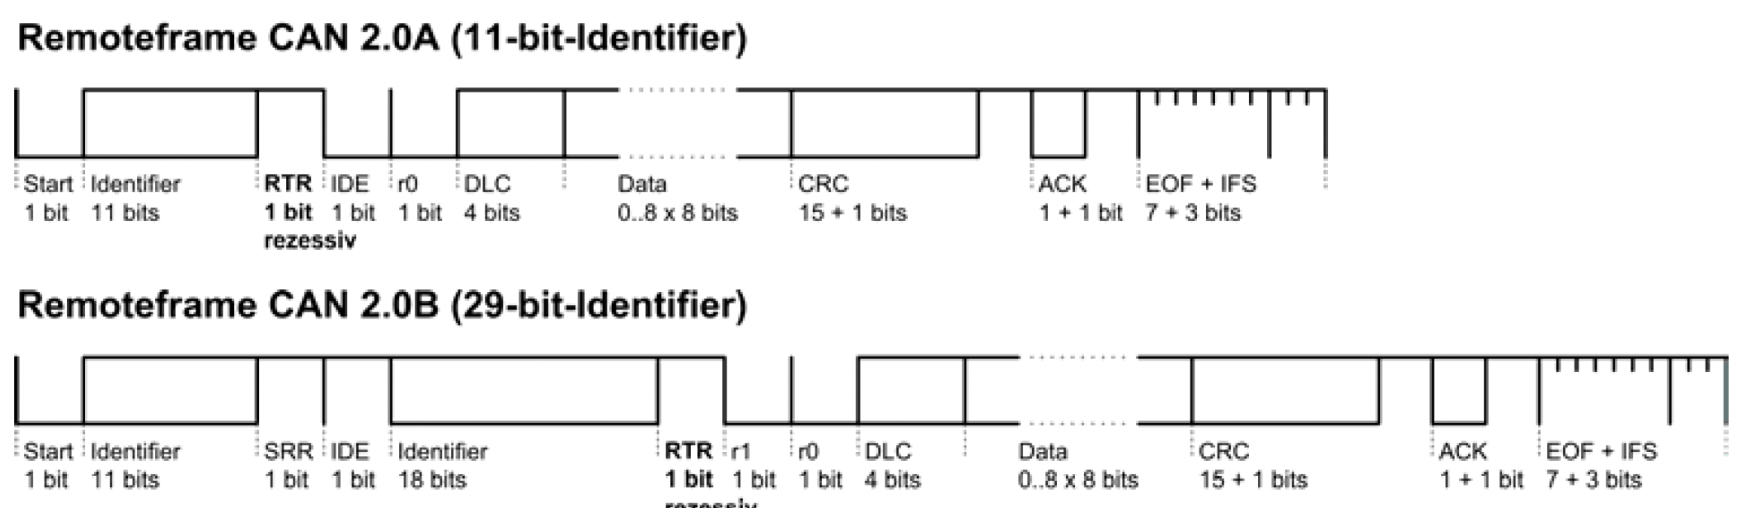
\includegraphics[width=\Bildbreite]{Grafiken/CAN_Telegrame-crop.pdf}
    \caption{CAN-Telegramme \cite{lawrenzCANControllerArea2016}}
    \label{fig: CAN_Telegramme}
    \end{figure}    

Der erste Abschnitt ist das Arbitration-Feld, das zur Regelung des Buszugriffs benötigt wird (siehe Abbildung \ref{fig: CAN_Telegramme}).
Das Arbitration-Feld beginnt mit einem Startbit, das immer "low" (dominant) ist. Auf das Startbit folgt der 11 Bit lange Identifier, der den Inhalt und die Priorität des Telegramms enthält. Je höher der Wert des Identifiers, desto niedriger ist die Priorität des Telegramms. Das letzte Bit im Arbitration-Feld ist das Remote Transmission Request-Bit (RTR-Bit), welches angibt, ob das Telegramm Daten enthält oder ob der entsprechende Teilnehmer aufgefordert wird, ein Telegramm zu senden.

Auf das Arbitration-Feld folgt das Control-Feld. Dieses beginnt mit dem Identifier Extension Bit (IDE-Bit), das bei Standard-Frames auf "low" (dominant) gesetzt ist. Das folgende r0-Bit ist reserviert. Im 4 Bit langen DLC-Bereich des Control-Feldes ist die Länge der nachfolgenden Daten festgelegt.

Das darauf folgende Data-Feld kann 0 bis 8 Byte lang sein und enthält die eigentlichen Nutzdaten des Telegramms.

Nach dem Data-Feld folgt das 16 Bit lange CRC-Feld, welches zur Fehlererkennung dient. Durch das CRC-Feld können Einzelbitfehler bis zu einer Anzahl von 6 und aufeinanderfolgende Bitfehler (Burst-Errors) bis zu einer Länge von 15 Bit erkannt werden. Eine genauere Ausführung zur Fehlererkennung erfolgt im Kapitel Fehlermanagement.

Nach dem CRC-Feld folgt das ACK-Feld mit einer Länge von 2 Bit. Die Busteilnehmer, die eine gesendete Nachricht korrekt empfangen haben, bestätigen dies, indem sie einen dominanten Pegel auf dem ersten Bit des ACK-Feldes senden. Der Sender der Nachricht interpretiert einen nicht-dominanten Pegel als Fehler. Das letzte Bit im ACK-Feld ist der ACK-Delimiter, der immer rezessiv ist.

Das letzte Feld ist das EOF-Feld (End-Of-Frame-Feld), das mit einer Länge von 7 Bit das Ende des Telegramms markiert. Im EOF-Feld sind alle Bits rezessiv.

Um den Busteilnehmern nach einem Telegramm Zeit zum Abspeichern des Telegramms zu geben, folgt der sogenannte Interframe Space (IFS) mit einer Länge von 3 Bit. Auch hier sind alle Bits rezessiv.

Durch die aufeinander folgenden rezessiven Bits wird signalisiert, dass der Bus aktuell nicht genutzt wird. Ein neuer Teilnehmer kann dann durch ein Startbit ein neues Telegramm senden.

\subsection{Besonderheiten von langen CAN-Telegrammen}
Wie in Abbildung \ref{fig: CAN_Telegramme} zu sehen, folgt bei einem langen Datentelegramm nach den ersten 11 Bits des Identifiers ein SRR-Bit (Substitute Remote Request) anstelle des RTR-Bits bei kurzen Telegrammen. Das darauf folgende IDE-Bit liegt bei langen Telegrammen an derselben Stelle wie im kurzen Telegramm. Jedoch ist dieses IDE-Bit im langen Telegramm rezessiv und kündigt damit an, dass weitere 18 Identifier-Bits folgen. Nach diesen Bits ist der Identifier im Extended-CAN-Frame vollständig, und danach folgt ein RTR-Bit mit derselben Funktion wie im kurzen Telegramm.

Auf das RTR-Bit folgt im langen Telegramm das 6 Bit lange Control-Feld, in dem die ersten zwei Bits, r0 und r1, reserviert sind. Auf diese folgen 4 Bits, die die Längeninformation der darauffolgenden Daten enthalten.









